\chapter{Planificación e seguimento}
\minitoc
% \label{chap:Planificacioneseguimento}
% \vspace{0.5cm}

%%%%%%%%%%%%%%%%%%%%%%%%%%%%%%%%%%%%%%%%%%%%%%%%%%%%%%%%%%%%%%%%%%%%%%%%%%%%%%%%
% Objetivo:                        %
%%%%%%%%%%%%%%%%%%%%%%%%%%%%%%%%%%%%%%%%%%%%%%%%%%%%%%%%%%%%%%%%%%%%%%%%%%%%%%%%

  \lettrine{N}{este} capítulo detallaremos a planificación e o seguimento 
do proxecto, un proxecto que por diversas circunstancias de dividíu 
principalmente en tres grandes etapas, as dúas primeiras mentres VACmatch era 
unha iniciativa emprendedora e a última durante a cal se comezou unha conversión 
da iniciativa cara un proxecto comunitario de software libre.

\santiagosays{Ao principio tamén quería ser un proxecto de SwL, non?
  Igual isto hai que explicalo mellor nalgures. Porque antes deste
  capítulo todo é falar de VACmatch como unha iniciativa emprendedora;
  e, bueno, agora mesmo non estamos emprendendo moito nin moi lean.}

  \begin{description}
    \item [Agosto 2015 - Outubro 2015] VACmatch. Validación de negocio.
    \item [Outubro 2015 - Xaneiro 2016] VACmatch. Desenvolvemento de produto.
    \item [Xaneiro 2016 - Xuño 2016] De empresa a comunidade.
  \end{description}


  \section{Validación de negocio (Xullo 2015 -- Novembro 2015)}
  A duración de esta etapa é de aproximadamente 4 meses e ven determinada polos 
primeiros pasos de VACmatch como iniciativa empresarial e que levan a orientar 
o desenvolvemento do produto cara o cliente, comezando con unha serie de 
prototipos para coñecer as suas necesidades e validar a idea de 
negocio.

  Durante o primeiro mes planificase a realización de un prototipo visual co 
fin de comprobar a usabilidade e consolidar os requisitos dos clientes.
  De seguido, plantéxase crear un pequeno prototipo funcional, un Mínimo 
Producto Viable (MVP) na metodoloxía Lean Startup, co obxectivo de testear as 
necesidades dos clientes e definir o produto final a desenvolver.

    \subsection{I Torneo VACmatch}
    Durante este periodo tamén se planificou a organización dun torneo de 
fútbol sala a finais do mes de Outubro coa idea de probar en un entorno real 
e controlado, os primeiros prototipos desenvoltos.

    Finalmente participaron 6 equipos e mais de 50 persoas durante dous días.

    \begin{figure}[h!]
          \begin{center}
          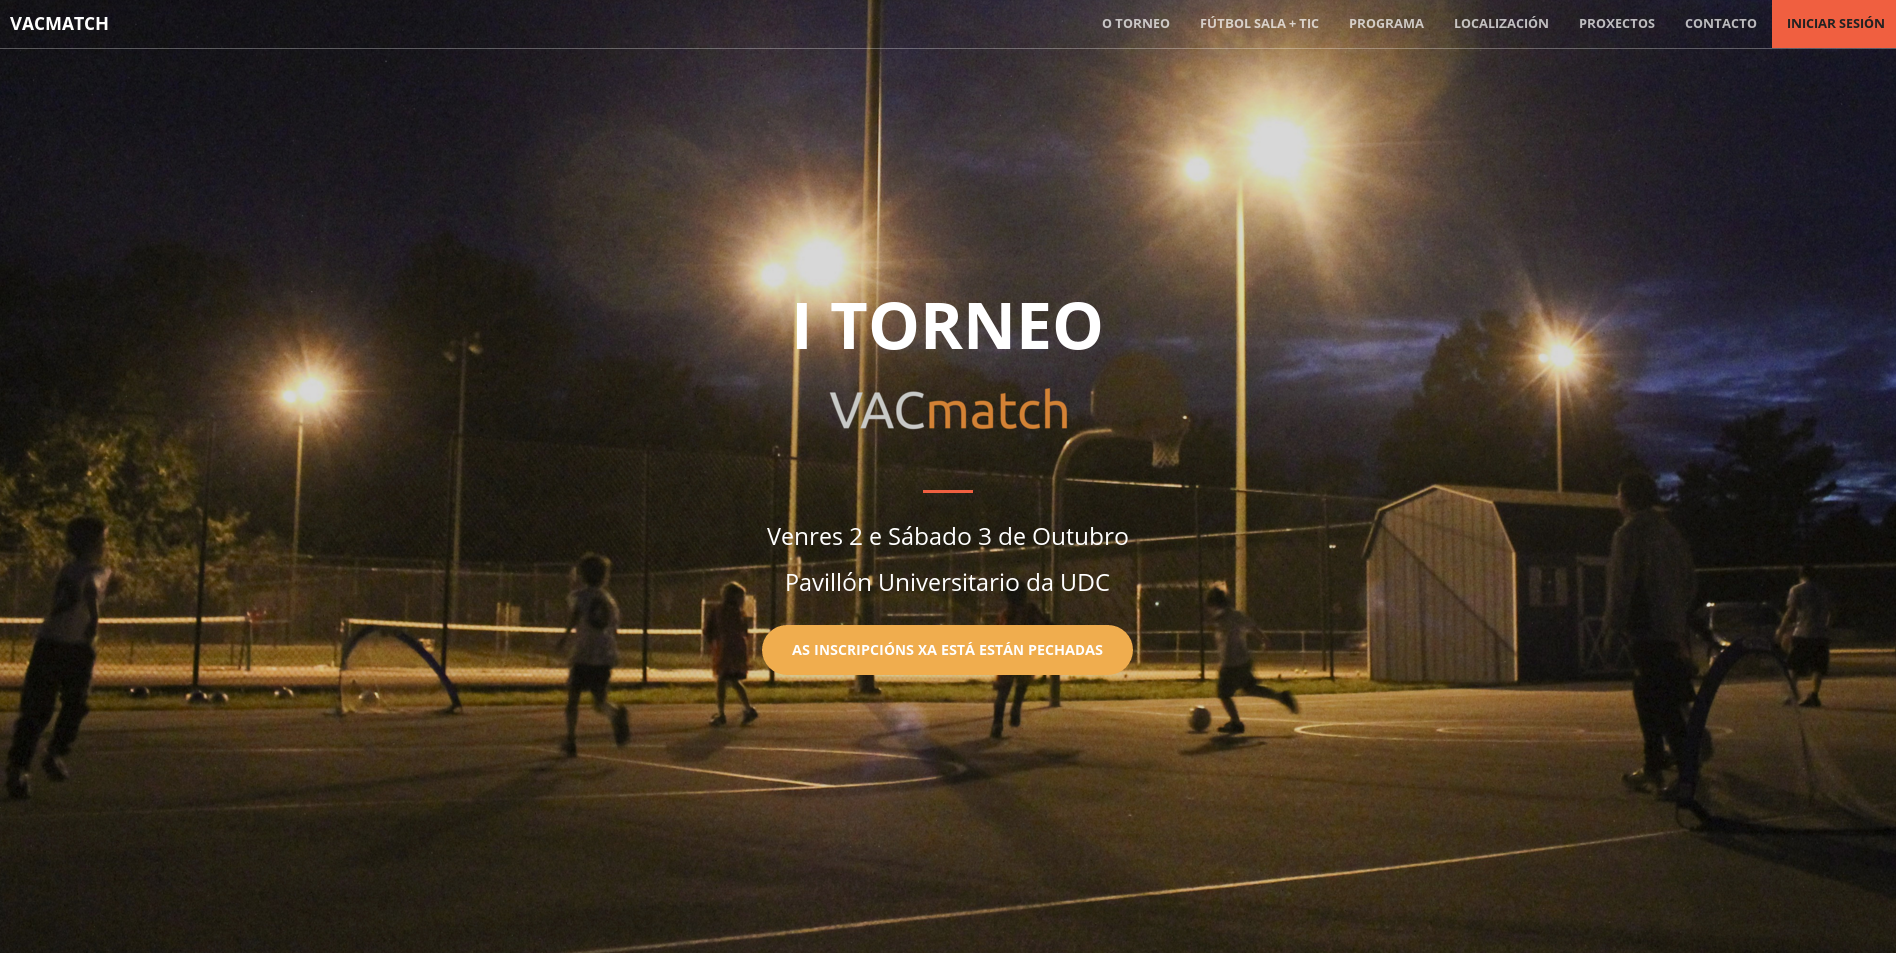
\includegraphics[width=\textwidth]{./img/torneo_vacmatch.png}
          \caption{Web do I Torneo VACmatch}
          \end{center}
    \end{figure}

    \subsection{Prototipo visual}

      \subsubsection{Planificación temporal}
      Esta iteración dura un total de 4 semanas de desenvolvemento entre o 15 
de Xullo e o 16 de Agosto e realizase unha visita semanal ao cliente para obter 
feedback e mostrarlle a evolución do prototipo.

      \subsubsection{Definición da iteración}
      Durante este periodo de un mes de duración planificouse o desenvolvemento 
de unha aplicación moi sinxela e sen funcionalidade, que únicamente permitise 
analizar a usabilidade do sistema e comprobar si é factible adaptar o proceso 
de creación de un acta deportiva, a unha aplicación móbil.

    Así mesmo, ao longo do período realizaranse ata tres visitas a federación 
coa que se traballou dende o primeiro momento para comprobar a experiencia de 
un futuro usuario real da aplicación e obter feedback para futuras melloras.

      \subsubsection{Revisión e feedback}
      Durante as visitas as federacións obtivéronse diversas prospostas que 
levaron a adaptar o prototipo:

      \begin{itemize}
        \item Facer interactiva a aplicación e non mostrar grandes táboas con 
datos.
        \item Todas as accións deben xirar ao redor da acta.
        \item Crear partidos cando non hai cobertura.
      \end{itemize}

      \subsubsection{Tarefas e seguimento}

      As tarefas de esta iteración son as seguintes:

      \begin{itemize}
        \item Crear esqueleto da aplicación.
        \item Como árbitro quero poder consultar as próximas actas a 
cubrir.
        \item Como árbitro quero poder consultar as actas xa cubertas.
        \item Como árbitro quero poder editar un acta.
        \item Como árbitro quero poder ver un acta.
        \item Como árbitro quero poder ver os xogadores de ambos equipos.
        \item Como árbitro quero poder engadir un evento.
        \item Como árbitro quero poder rematar ou suspender un partido.
        \item Como árbitro quero poder logearme.
        \item Como árbitro quero poder seleccionar cales xogadores de cada 
equipo se atopan no encontro.
        \item Como árbitro quero poder borrar un evento.
        \item Estudio sobre React e Flux.
       \end{itemize}

      Planificaronse X horas, fixéronse X por isto

    \subsection{MVP funcional}

      \subsubsection{Planificación temporal}
      Esta iteración dura un total de 3 meses e desenvólvese entre o 16 de 
Agosto e o 15 de Novembro, realizando múltiples visitas as federacións.

      \subsubsection{Definición da iteración}
      Unha vez finalizadas as probas visuais e de usabilidade procedese 
a planificar o desenvolvemento para adaptar o prototipo e engadirlle 
funcionalidade sinxela, sen validacións e sen funcionalidade offline, co 
obxectivo de obter un prototipo funcional que poida ser utilizado por usuarios 
reais nun entorno controlado.

      Engadirase funcionalidade para as vistas creadas na iteración anterior, 
comezando polo listado de actas pendentes e rematadas e diversos compoñentes 
xenéricos como os que se utilizan para listar xogadores e outros elementos como 
poden ser as actas.

      Únicamente se engadirá a funcionalidade básica imprescindible para 
xestionar un encontro, excluindo requisitos como a sinatura de actas ou a 
creación offline das mesmas co fin de axilizar as primeiras probas.

      Durante a iteración tamén se farán visitas a federación para mostrar o 
estado do desenvolvemento e para buscar que tamén árbitros reais vexan os 
progresos e proporcionen feedback.

      Unha vez rematada a iteración realizarase o torneo onde probar o 
prototipo desenvolto nun caso real.

      \subsubsection{Revisión e feedback}
      Durante as visitas as federacións obtivéronse múltiples propostas e 
melloras, moitas das cales será incorporadas ao backlog do proxecto mentres que 
outras serán rexeitadas polo momento ao non considerarse prioritarias ou por 
ser casos de usos moi concretos para esa federación e dificilmente 
extrapolables a outras.

      \textbf{Listaxe de tarefas engadidas ao backlog}.
        \begin{itemize}
          \item Meter xogadores manualmente xa que poden non terse creado no 
sistema de xestión.
          \item Poder ver os eventos de forma sinxela dende a vista de fin de 
partido para que os equipos vexan o que están firmando.
         \item Editar dorsal dos xogadores xa que poden cambiar.
         \item Ter opción de non poñer motivo para as tarxetas.
         \item Mostrar foto de xogador ao engadir un evento.
        \end{itemize}

      \textbf{Listaxe de tarefas rexeitadas polo momento}.
        \begin{itemize}
         \item Ao marcar doble amarela, avisar da expulsión. Moi concreta para 
un deporte, non se implementa de momento.
         \item Mostrar confirmación de que se engadíu un evento.
         \item Avisar aos delegrados/personal do clube cando se sube un acta.
         \item Posibilidade de que o árbitro engada un anexo na casa a acta en 
lugar de escribir as incidencias.
        \end{itemize}

      \subsubsection{Tarefas e seguimento}

            \begin{itemize}
        \item Como árbitro quero poder cargar a lista de actas pendentes.
        \item Como árbitro quero poder cargar a lista de actas rematadas.
        \item Como árbitro quero poder ver os datos dun partido.
        \item Como árbitro quero poder ver a lista de xogadores dun equipo.
        \item Como árbitro quero poder seleccionar os xogadores presentes no 
partido.
        \item Como árbitro quero poder engadir un gol a un xogador.
        \item Como árbitro quero poder engadir unha falta a un xogador.
        \item Como árbitro quero poder engadir unha tarxeta (amarela ou 
vermella) a un xogador.
        \item Como árbitro quero poder ver a lista de eventos de un partido.
        \item Como árbitro quero poder borrar eventos de un partido.
        \item Como árbitro quero poder engadir incidencias a un partido.
       \end{itemize}




  \section{Desenvolvemento de produto (Novembro 2015 -- Xaneiro 2016)}
  Tras analizar os problemas e os erros cometidos durante a realización do I 
Torneo VACmatch, e concretamente no funcionamento da aplicación móbil durante o 
mesmo, decidíuse comezar novamente dende o principio un proxecto novo en lugar 
de facer unha refactorización do prototipo.

    Durante este tempo decidimos inscribir o proxecto no ``Concurso 
Universitario de Software Libre'' o que incentivou a comezar a escribir un 
blog técnico, a través da conta de Medium de VACmatch, no que contar os avances 
que van sucedendo durante o desenvolvemento do proxecto.

    \subsection{Participación na I Lonxa de Financiamento Responsable}
    Durante este tempo tamén cómpre destacar a participación de VACmatch na I 
Lonxa de Financiamento Responsable en Galicia, permitíndonos presentar o noso 
proxecto ante diversos inversores preocupados pola responsabilidade social das 
empresas.

    Foi unha experiencia única que nos permitíu introducirnos por primeira vez 
no mundo da inversión en startups e coñecer aos diversos proxectos que se 
presentaron.

    \begin{figure}[h!]
          \begin{center}
          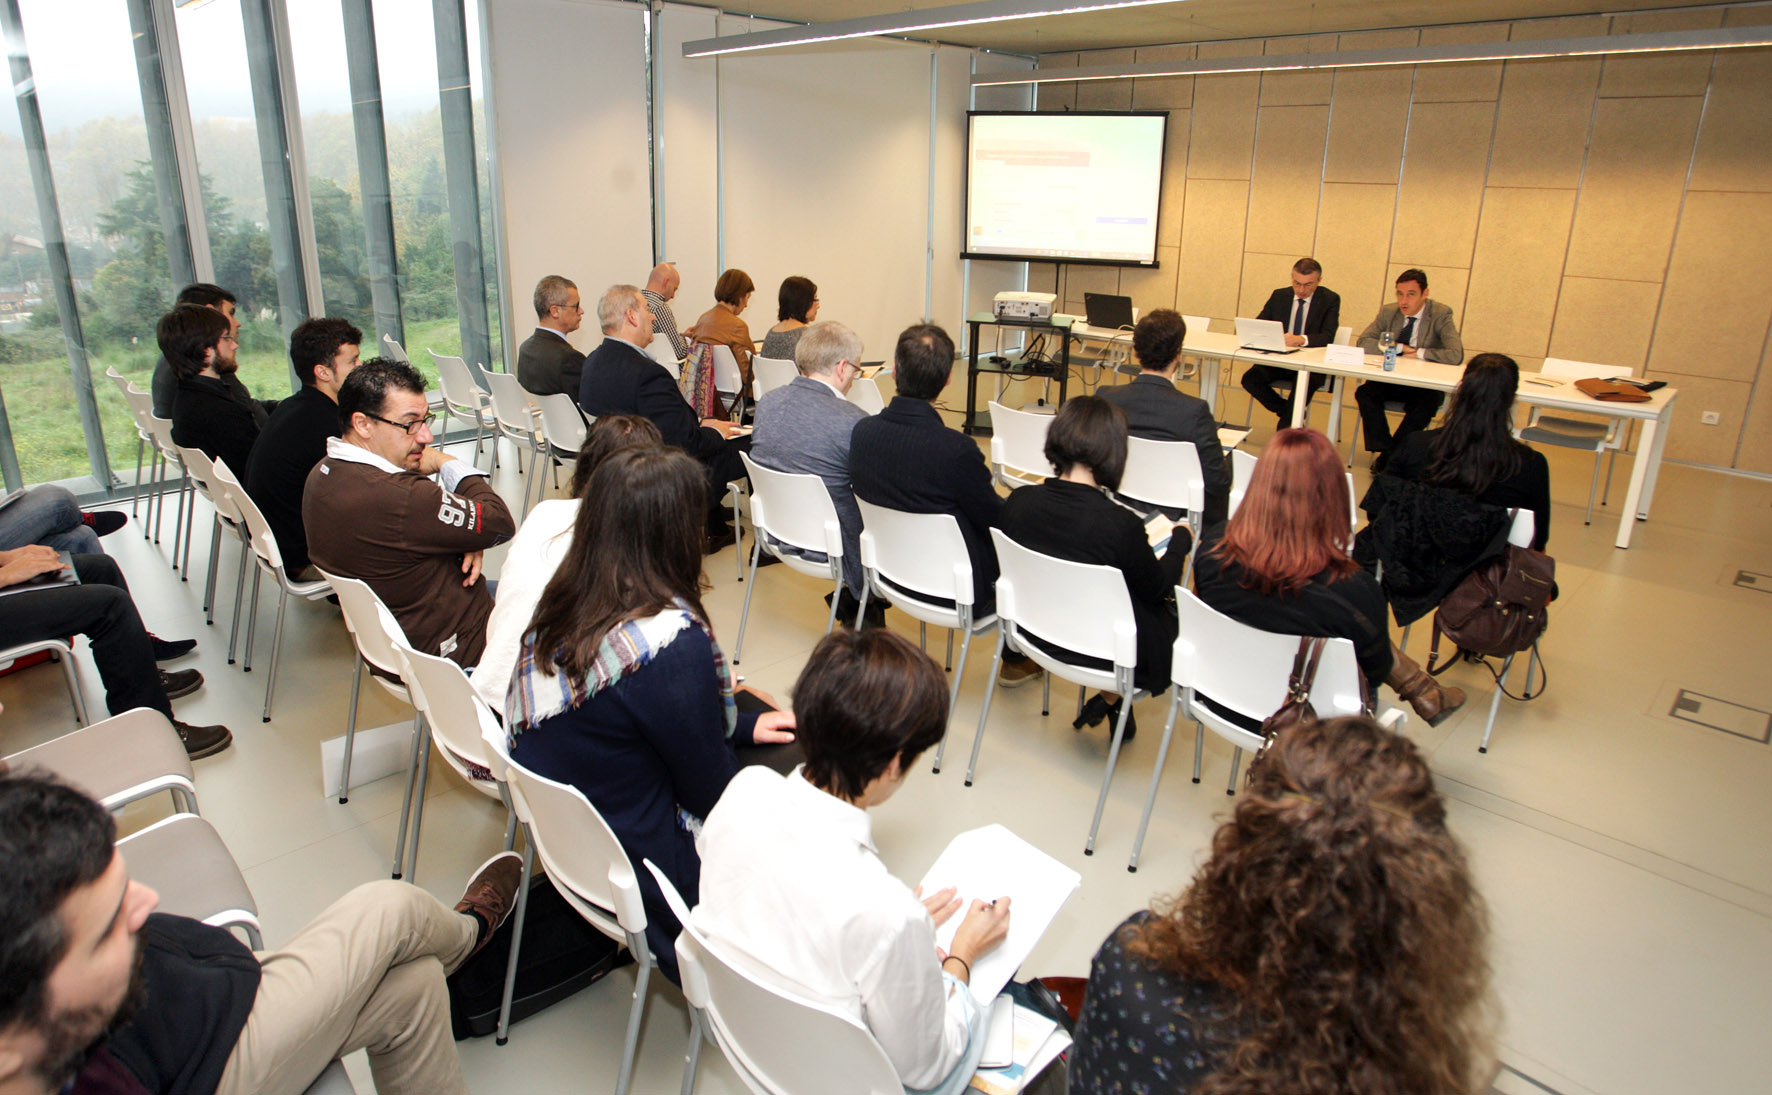
\includegraphics[width=0.8\textwidth]{./img/inversion_responsable.jpg}
          \caption{I Lonxa de Financiamento Responsable}
          \end{center}
    \end{figure}

    \subsection{1ª iteración. Creación do proxecto}

      \subsubsection{Planificación temporal}
  Esta iteración transcorre entre o día 1 e o 15 do mes de Novembro de 2015

      \subsubsection{Definición da iteración}
      A presente iteración centrase en comezar o desenvolvemento da 
aplicación pensando dende o primeiro momento no funcionamento tanto online 
como offline e controlando os posibles conflictos que poidan suceder entre os 
datos.

      Comézase co estudo da tecnoloxía en profundidade xa que os 
prototipos non utilizaban nin Reflux nin PouchDB e simplemente enviaban os 
datos a unha API remota.

      Crease tamén o proxecto base engadindo a licencia e definese o modelo de 
datos que vai cambiar bastante do modelo inicial, pensando para unha base de 
datos relacional que é a que podíamos atopar na API remota.

      É por iso que os datos serán desnormalizados e pasarán a almacenarse en 
documentos en lugar de en táboas.

      Por último comezase a implementación do listaxe de actas a cubrir e de un 
boton para engadilas e eliminalas de xeito sinxelo para facer as primeiras 
probas.
      \subsubsection{Revisión e feedback}
      Durante esta iteración analizáronse os problemas detectados durante o 
torneo, optando por comezar a implementación do proxecto dende cero como se 
comentóu anteriormente.

      Tamén se realizaron diversas publicacións do blog para comentar a 
realización do torneo e sobre todo analizar aspectos como a elección 
tecnolóxica, a metodoloxía de desenvolvemento e as próximas funcionalidades a 
abordar.

      \subsubsection{Tarefas e seguimento}

        \begin{itemize}
         \item Definir modelo de datos.
         \item Deseñar mockups finais.
         \item Crear proxecto base.
         \item Estudio da tecnoloxía. React, Reflux, PouchDB, Redmine
         \item Crear modelos en PouchDB.
         \item Como árbitro quero poder obter a lista de actas a cubrir.
         \item Permitir crear e borrar actas para tarefas de test.
         \item Engadir licencia e Readme
        \end{itemize}


    \subsection{2ª iteración. Xestión de actas}

      \subsubsection{Planificación temporal}
      A iteración comeza o día 16 de Novembro e remata o día 30 do mesmo mes.

      \subsubsection{Definición da iteración}
        Nesta 2º iteración planifícase o desenvolvemento das páxinas principais 
e básicas para a xestión da acta dun encontro.

      As funcionalidades que se abordarán neste sprint centranse principalmente 
na vista na que se mostra o resumo actual da acta así como o control do tempo, 
co fin de permitir xestionar o encontro en tempo real de forma interactiva.

      \subsubsection{Revisión e feedback}
      Ao non realizar ningunha visita a federacións, non se obtivo feedback 
pero si é importante mencionar que se produciron retrasos e polo tanto varias 
tarefas foron transladadas ao seguinte sprint de desenvolvemento.

      \subsubsection{Tarefas e seguimento}

        \begin{itemize}
         \item Como árbitro quero ver o resumo da acta.
         \item Como árbitro quero controlar o tempo do partido.
         \item Como árbitro quero manter o tempo do partido aínda que cambie de 
páxina.
        \end{itemize}

        \todo{Mencionar tarefas retrasadas a que pasan ao seguinte sprint}

    \subsection{3ª iteración. Eventos}

      \subsubsection{Planificación temporal}
      Dende o 30 de Novembro ata o 13 de Decembro.

      \subsubsection{Definición da iteración}
      Esta iteración céntrase principalmente na xestión de eventos dos 
encontros, tarefas que requiren unha forte planificación e análise xa que se 
busca que ditos eventos sexan o máis xenéricos posibles e facilmente adaptables 
aos diversos deportes.

      Da mesma forma se plantexa crear tipos de eventos que modifiquen tamén a 
propia acta, actualizando na mesma tanto o resultado como as faltas cometidas.

      Por último incorporase tamén na iteración convocar e editar persoas dun 
equipo así como algún pequeno erro detectado na última iteración.

      \subsubsection{Revisión e feedback}

      \subsubsection{Tarefas e seguimento}

        \begin{itemize}
          \item Como árbitro quero poder engadir un evento.
          \item Como árbitro quero ver a lista de xogadores para asignar un 
evento.
          \item Como árbitro quero poder confirmar engadir un evento.
          \item Como árbitro quero engadir unha causa a un evento.
          \item Cómo árbitro quero poder ver a lista de eventos de un partido.
          \item Como árbitro quero que se xeneren eventos de comezo e fin de 
partido.
          \item Como árbitro quero que se xeneren eventos ao cambiar de parte.
          \item Como árbitro quero que se actualice o resultado ao engadir un 
gol.
          \item Como árbitro quero que se actualicen as faltas automáticamente.
          \item Como árbitro quero poder convocar e desconvocar xogadores.
          \item Como árbitro quero poder cambiar o dorsal de un xogador nun 
partido determinado.
          \item Como árbitro quero poder borrar un evento.
          \item Como árbitro quero ver a lista de eventos de un partido 
ordenada por tempo e parte.
          \item Mostrar únicamente xogadores convocados ao engadir un evento.
          \item Como árbitro quero que ao borrar un evento se actualicen os 
resultados e as faltas na Acta.
          \item Erro: Cando non hai ningún evento de cambio de parte hai un 
error.
          \item Erro: Corexir erro cando se engade un evento con causa.
        \end{itemize}

    \subsection{4ª iteración. Xestión de usuarios e creación offline de actas}
    
    login, logout, metese staff, crear actas offline
    Memoria, 3 primeros apartados
      \subsubsection{Planificación temporal}
      Esta iteración ten lugar entre o 14 e o 30 de Decembro de 2015.

      \subsubsection{Definición da iteración}
      Esta iteración centrase na autenticación da aplicación que debe integrar 
unha base de datos remota para que os árbitros poidan conectarse co seu usuario 
e tamén inclúe a creación e edición manual de actas que en anteriores 
iteracións foi engadida únicamente para probas internas pero sen 
realizar as comprobacións necesarias.

      Tamén se planifican tarefas para comezar as primeiras partes da memoria 
do proxecto que incluen a introdución, o estado da arte os fundamentos 
tecnolóxicos.

      \subsubsection{Revisión e feedback}
      Post no blog -> fundamentos tecnolóxicos e estado do proxecto.

      \subsubsection{Tarefas e seguimento}

        \begin{itemize}
          \item Como usuario quero poder facer log in.
          \item Engadir diferenciación entre Persoal e Xogadores.
          \item Como usuario quero poder facer log out.
          \item Como árbitro quero poder crear un partido manualmente.
          \item [Memoria] Definir introdución.
          \item [Memoria] Estado da arte.
          \item [Memoria] Fundamentos tecnolóxicos.
          \item [Memoria] Engadir modelo.
          \item Como árbitro quero poder editar un acta creada dende o móbil.
          \item Erro: Correxir erro coa variable dialogIsOpen ao editar o 
dorsal de un xogador.
        \end{itemize}

    \subsection{5ª iteración. Sinaturas}
    Sinaturas con PIN, engadir incidencias
    do sprint anterior: crear usuario, crear árbitro ao crear user

      \subsubsection{Planificación temporal}
      Esta iteración comeza o día 1 de Xaneiro de 2016 e remata o día 8.

      \subsubsection{Definición da iteración}
      A presente iteración centrase na última vista da aplicación, a que 
permite xestionar a finalización do encontro dando a posibilidade de asinar a 
acta e engadir comentarios por parte do árbitro.

      Na última iteración detectaronse varias melloras a incluir como facer que 
por defecto as contas creadas dende a aplicación móbil sexan todas de tipo 
árbitro e a todas as actas que cree esa conta, se engada a dito usuario como 
árbitro do encontro.

      \subsubsection{Revisión e feedback}
      

      \subsubsection{Tarefas e seguimento}

        \begin{itemize}
         \item Como árbitro quero poder asinar un acta.
         \item Como árbitro quero que unha ou varias persoas convocadas de cada 
equipo poidan asinar un acta.
         \item Como árbitro quero poder engadir comentarios a un acta.
         \item Como árbitro quero poder borrar un xogador da lista de 
convocados.
         \item Crear un árbitro ao crear un novo usuario na aplicación móbil.
         \item Engadir o árbitro que ten o usuario asignado nas actas que crea.
        \end{itemize}

  \section{De empresa a comunidade (Xaneiro 2016 -- Maio 2016)}
  Durante o mes de Xaneiro de 2016 decidíuse abandonar o proxecto de VACmatch 
como iniciativa empresarial por diversos motivos e continuar con él únicamente 
como proxecto comunitario de software libre.

  Motivado por isto, producíuse un parón de aproximadamente un mes de duración 
e ao mesmo tempo comezouse a traballar nunha empresa externa polo que durante 
este período diminuíu considerablemente o tempo dispoñible para continuar co 
proxecto.

    \subsection{6ª e 7ª iteración. Optimización e melloras}
    Motivado pola inestabilidade xerada polos cambios mencionados anteriormente,
non se realizou unha correcta planificación da 6ª iteración e finalmente non su 
realizóu ningunha tarefa polo que se decidíu unir ambas iteracións.

      \subsubsection{Planificación temporal}
      Estas iteracións comezan o 14 de Febreiro de 2016 e rematan o 29 de 
Febreiro.

      \subsubsection{Definición da iteración}
      Durante esta iteración planificouse unha importante refactorización de 
código co fin de simplificar certas partes do código e facilitar o mantemento 
da aplicación así como revisar a forma na que se crean os identificadores dos 
obxectos en base de datos.

      \subsubsection{Revisión e feedback}


      \subsubsection{Tarefas e seguimento}

        \begin{itemize}
         \item Refactorizar servicios.
         \item Crear clases para cada entidade.
         \item Revisar cómo se crean os identificadores dos obxectos en base de 
datos.
        \end{itemize}

    \subsection{8ª iteración. Testing e integración continua}

      \subsubsection{Planificación temporal}
      A iteración transcorre entre os días 1 e 14 de Marzo.

      \subsubsection{Definición da iteración}
      Decidíuse engadir tests unitarios para previr futuros erros e facilitar o 
mantemento da aplicación xa que en todo proxecto de certa embergadura, e máis 
en proxectos libres nos que calquera pode colaborar, é importante asegurar que 
os novos cambios que se engadan, non xeneren problemas no funcionamento da 
aplicación.

      Relacionado con este tema tamén se planificou a integración do 
repositorio de código con unha ferramenta de integración continua que facilite 
a execución de este tipo de provas, en este caso Travis CI.

      \subsubsection{Revisión e feedback}

      \subsubsection{Tarefas e seguimento}

        \begin{itemize}
         \item Engadir tests aos servizos de Eventos, Persoas, Equipos e Actas.
         \item Engadir tests aos servizos de Auth, Árbitros e Sinaturas.
         \item Engadir integración continua con Travis CI.
         \item Engadir campos para confirmar contrasinal e código PIN ao crear 
un usuario.
        \end{itemize}

    \subsection{9ª e 10ª iteración. Inxección de dependencias}
    Motivado de novo pola falta de tempo para traballar no proxecto, decidíuse 
integrar de novo estas dúas iteracións.

      \subsubsection{Planificación temporal}
      Estas iteracións comezan o día 15 de Marzo e rematan o 25 de Abril.

      \subsubsection{Definición da iteración}
      Detectáronse erros en Travis xa que non detectaba erros nos tests polo 
que é o primeiro que había que corrixir.

      Tamén se decidíu crear unha barra de notificacións compartida para todos 
os compoñentes da aplicación e engadíronse estados diferentes para as actas co 
fin de mostrar cando non comezóu, cando se está a xogar e cando se rematóu o 
encontro.

      Pero a tarefa máis importante xurdíu ao aparecer un problema de 
denpendencias circulares que obrigóu a engadir unha factoría para realizar unha 
inxección de dependencias entre os servizos da aplicación xa que varios, 
dependían uns de outros.

      Finalmente planificouse tamén a corrección de diversos erros detectados 
na iteración anterior.

      \subsubsection{Revisión e feedback}

      \subsubsection{Tarefas e seguimento}

      \begin{itemize}
       \item Engadir textos de error na aplicación.
       \item Crear barra de notificacións para utilizar en calquera compoñente.
       \item Engadir DAOs.
       \item Engadir Inxección de Dependencias.
       \item Engadir estados na Acta.
       \item Erro: Como árbitro non debería poder convocar/borrar a un xogador 
que ten eventos asignados.
       \item Erro: Mostrar que o partido rematóu na acta.
       \item Erro: Correxir problema de dependencias circulares.
       \item Erro: Correxir erros varios derivados de engadir inxección de 
dependencias.
       \item Erro: Un evento de comezo de partido non se pode borrar si existe 
algún outro evento creado.
       \item Erro na xestión do estado da Acta.
       \item Erro: Travis CI non funciona correctamente
      \end{itemize}

    \subsection{Release 0.2.0: Usabilidade en menús}

      \subsubsection{Planificación temporal}
      Esta iteración transcorre entre o día 25 de Abril e o 9 de Maio.

      \subsubsection{Definición da iteración}
      Unha iteración con unha sola tarefa pero de un tamaño suficiente para 
cubrir a totalidade do sprint, centrada en engadir os enlaces que faltaban no 
menú lateral esquerdo e no superior dereito, certos botóns de retroceso e 
corexidos diversos erros menores.

      \subsubsection{Concurso Universitario de Software Libre}
      Así mesmo, durante este iteración recibíuse o ``Premio al mejor proyecto 
de tecnologías móviles`` do Concurso Universitario de Software Libre (CUSL), un 
concurso onde participaron máis de 75 estudantes de toda España e donde se 
expuxeron 47 proxectos de código libre.

      Fomos invitados a participar na fase final que tivo lugar os días 5 e 6 
de Maio na Universidade de Sevilla na que presentar o proxecto ante 
representantes de diversas empresas de software libre españolas que tamén 
participaron con diversas charlas sobre os seus modelos de negocio e as 
vantaxes do software libre a nivel empresarial.

      Foi unha gran experiencia a compartida con todos os finalistas e 
asistentes e, por suposto, os custes da viaxe foron subvencionados pola 
organización e o premio finalmente foi de 500 \euro{} en metálico.

    \begin{figure}[h!]
          \begin{center}
            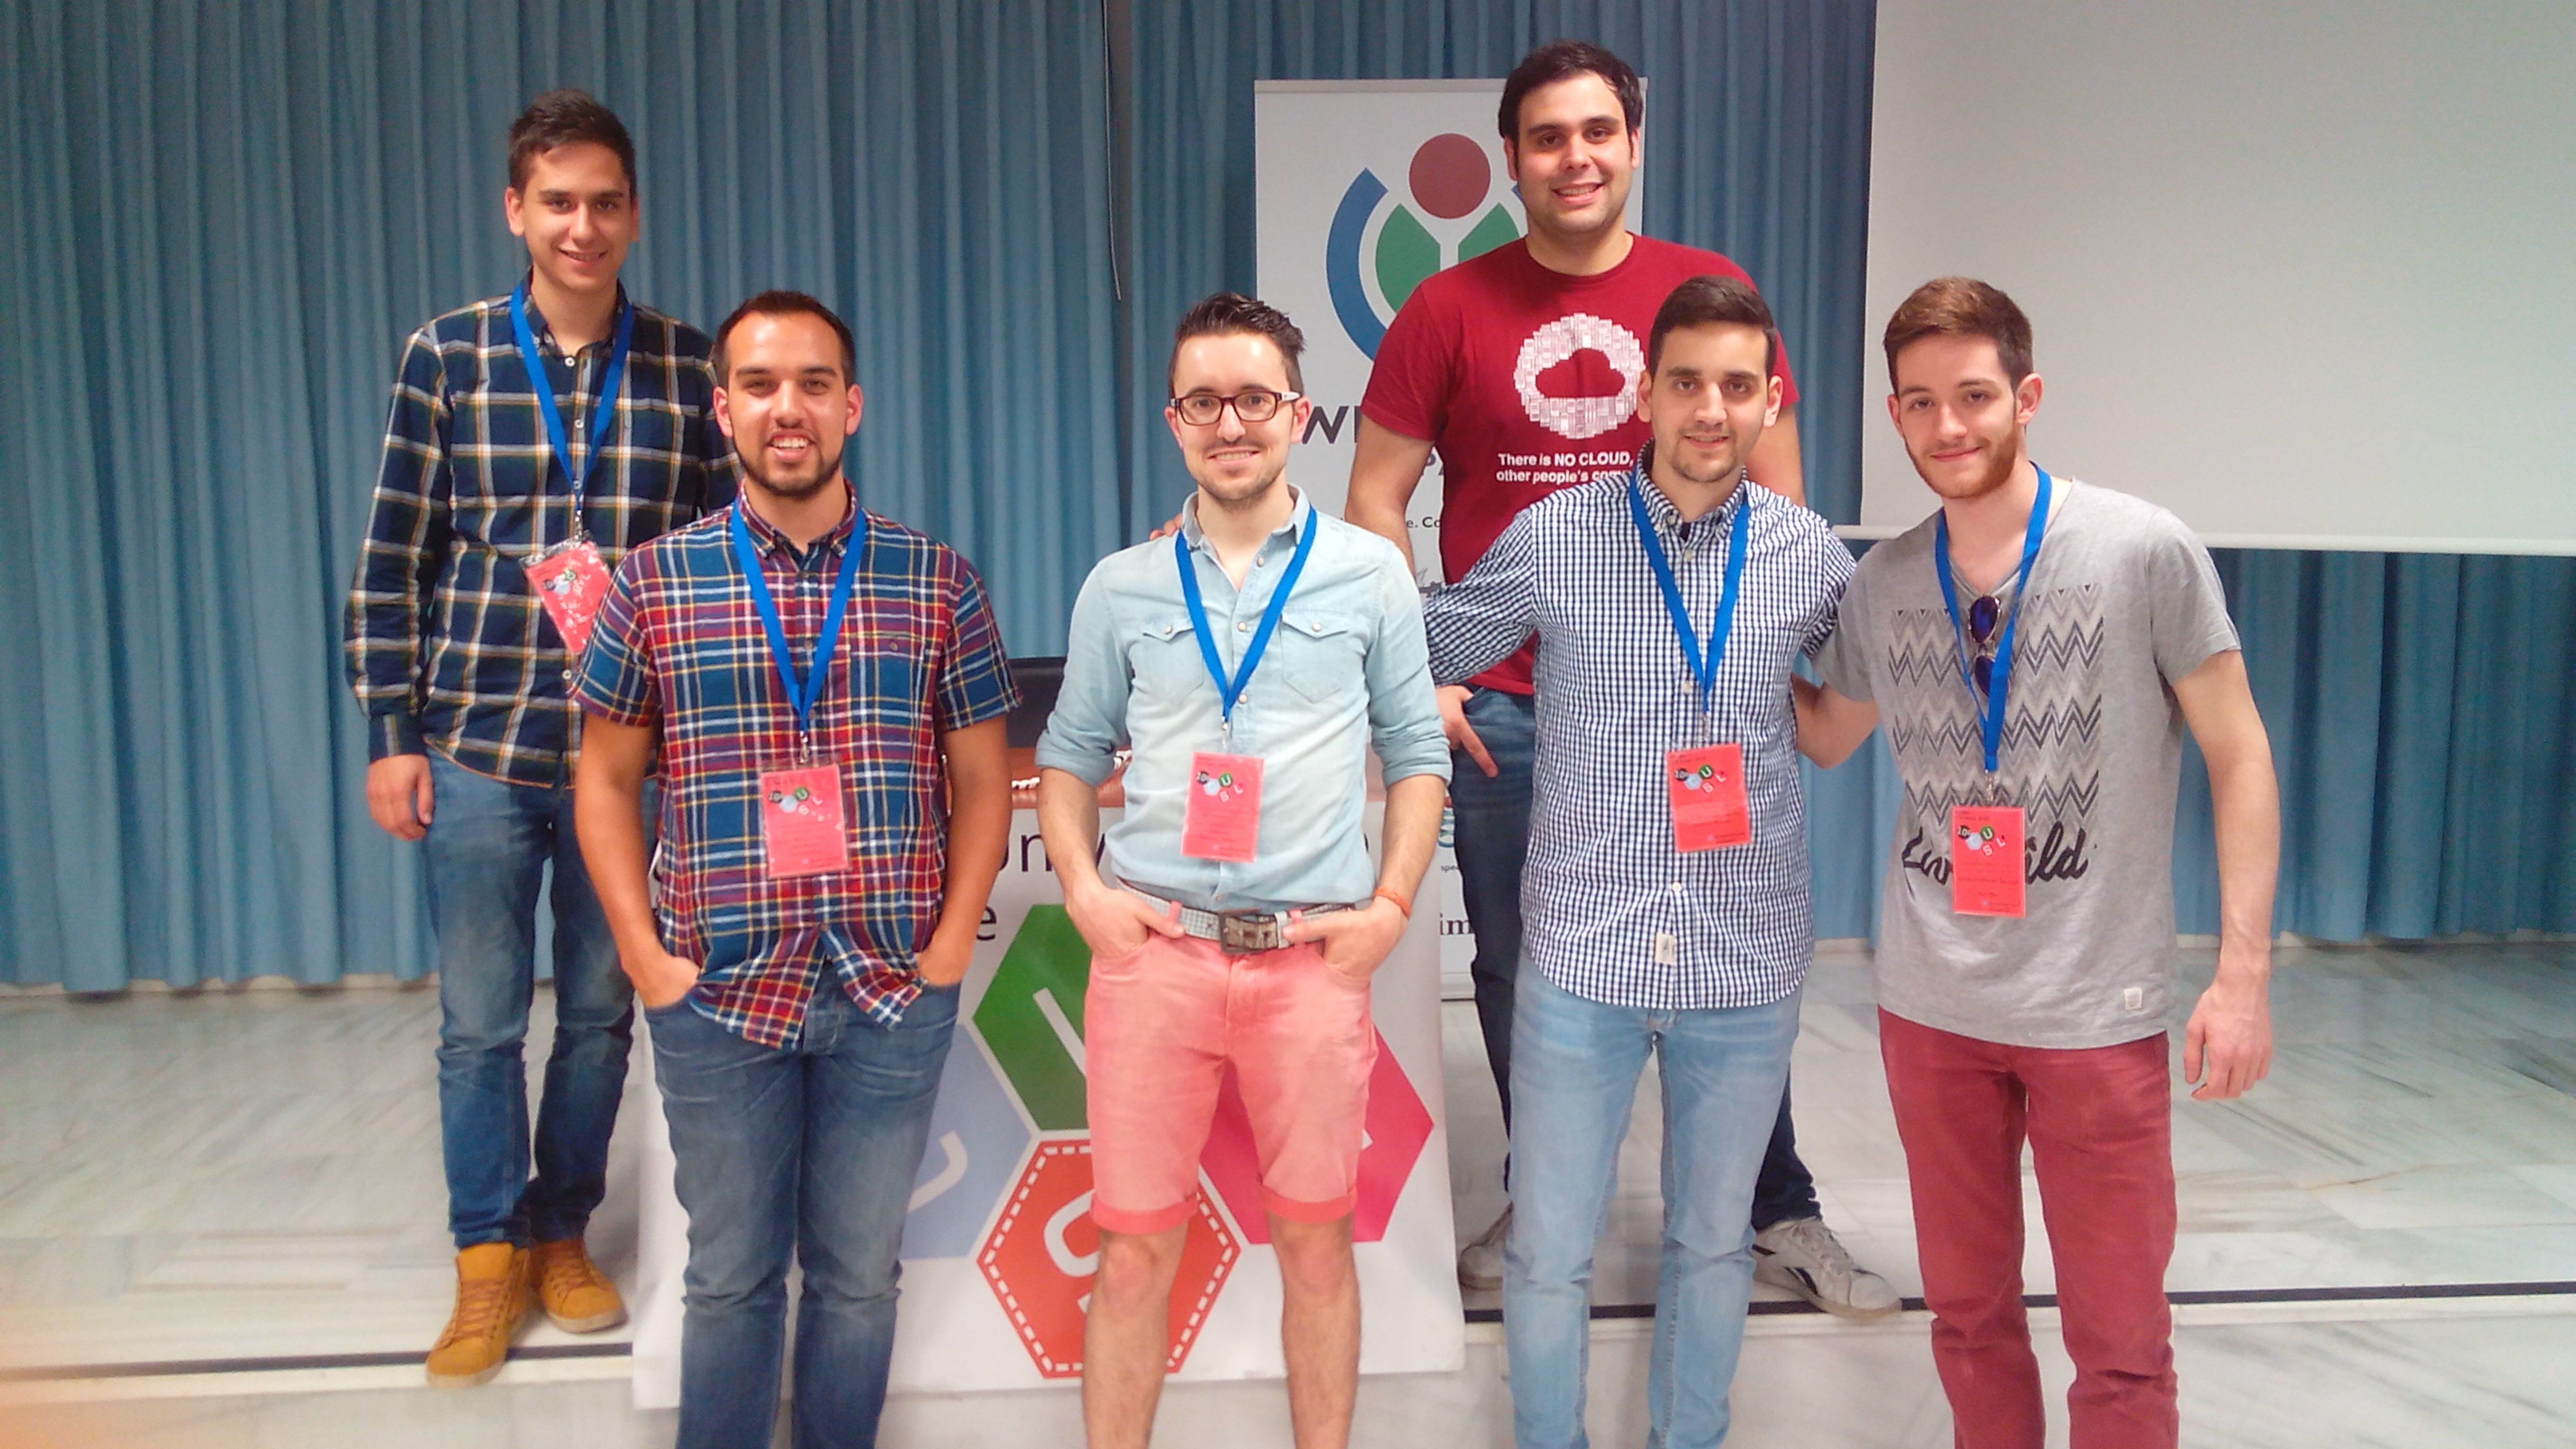
\includegraphics[width=0.8\textwidth]{./img/final_cusl.jpg}
            \caption{Finalistas CUSL}
          \end{center}
    \end{figure}

      \subsubsection{Revisión e feedback}

      \subsubsection{Tarefas e seguimento}
        \begin{itemize}
        \item Revisar os links nos menús e engadir información.
        \end{itemize}


    \subsection{Release 0.2.1: I18n e app híbrida}

      \subsubsection{Planificación temporal}
      Esta iteración comeza o día 9 e remata o 24 Maio.

      \subsubsection{Definición da iteración}
      A tarefa de maior tamaño que se planificou en esta iteración foi a 
internacionalización coa librería React Intl xa que supón modificar todas as 
vistas da aplicación.

      Posteriormente engadíuse Apache Cordova para permitir crear aplicacións 
híbridas que funcionen en diversos sistemas operativos móbiles e por suposto, 
tamén se incluíu no repositorio de código, a documentación sobre cómo arrancar 
unha base de datos CouchDB para utilizar como backend e sobre cómo realizar a 
compilación da aplicación para executar nun sistema operativo móbil.

      \subsubsection{Revisión e feedback}

      \subsubsection{Tarefas e seguimento}
        \begin{itemize}
        \item Engadir internacionalización.
        \item Crear app híbrida con Apache Córdova.
        \end{itemize}
%
% ----------- WORK IN PROGRESS
%
    \subsection{Release 0.2.2: Imáxe corporativa e revisión de erros}
    Imaxe corporativa VACmatch, bugfix
    Memoria a saco
      \subsubsection{Planificación temporal}
      \subsubsection{Definición da iteración}
      \subsubsection{Revisión e feedback}
      \subsubsection{Tarefas e seguimento}

    \subsection{Release 0.3.0: Usabilidade móbil e entrega continua}
    Por cordova: dialogos -> ventás, transición carga, migrar taiga.io, Travis + 
Docker
      \subsubsection{Planificación temporal}
      \subsubsection{Definición da iteración}
      \subsubsection{Revisión e feedback}
      \subsubsection{Tarefas e seguimento}


%%% Local Variables:
%%% mode: latex
%%% TeX-master: "../root"
%%% End:
